\documentclass[letterpaper]{article} % DO NOT CHANGE THIS
\usepackage[submission]{aaai2027}  % DO NOT CHANGE THIS
% The serif, sans-serif, and monospaced fonts are loaded automatically by
% aaai2027.sty (newtxtext, helvet, courier). DO NOT add \usepackage{times},
% \usepackage{helvet}, \usepackage{courier}, or any other font package.
\usepackage[hyphens]{url}  % DO NOT CHANGE THIS
\usepackage{graphicx} % DO NOT CHANGE THIS
\urlstyle{rm} % DO NOT CHANGE THIS
\def\UrlFont{\rm}  % DO NOT CHANGE THIS
\usepackage{natbib}  % DO NOT CHANGE THIS AND DO NOT ADD ANY OPTIONS TO IT
\usepackage{caption} % DO NOT CHANGE THIS AND DO NOT ADD ANY OPTIONS TO IT
\frenchspacing  % DO NOT CHANGE THIS
%
% These are recommended to typeset algorithms but not required. See the subsubsection on algorithms. Remove them if you don't have algorithms in your paper.
\usepackage{algorithm}
\usepackage{algorithmic}

%
% These are recommended to typeset listings but not required. See the subsubsection on listing. Remove this block if you don't have listings in your paper.
\usepackage{newfloat}
\usepackage{listings}
\DeclareCaptionStyle{ruled}{labelfont=normalfont,labelsep=colon,strut=off} % DO NOT CHANGE THIS
\lstset{%
	basicstyle={\footnotesize\ttfamily},% footnotesize acceptable for monospace
	numbers=left,numberstyle=\footnotesize,xleftmargin=2em,% show line numbers, remove this entire line if you don't want the numbers.
	aboveskip=0pt,belowskip=0pt,%
	showstringspaces=false,tabsize=2,breaklines=true}
\floatstyle{ruled}
\newfloat{listing}{tb}{lst}{}
\floatname{listing}{Listing}

%
% Recommended for better-looking tables
\usepackage{booktabs}

%
% Keep the \pdfinfo as shown here. There's no need
% for you to add the /Title and /Author tags.
\pdfinfo{
/TemplateVersion (2027.1)
}

% DISALLOWED PACKAGES
% \usepackage{authblk} -- This package is specifically forbidden
% \usepackage{balance} -- This package is specifically forbidden
% \usepackage{CJK} -- This package is specifically forbidden
% \usepackage{float} -- This package is specifically forbidden
% \usepackage{flushend} -- This package is specifically forbidden
% \usepackage{fullpage} -- This package is specifically forbidden
% \usepackage{geometry} -- This package is specifically forbidden
% \usepackage{hyperref} -- This package is specifically forbidden
% \usepackage{navigator} -- This package is specifically forbidden
% (or any other package that embeds links such as navigator or hyperref)
% \usepackage{indentfirst} -- This package is specifically forbidden
% \usepackage{layout} -- This package is specifically forbidden
% \usepackage{multicol} -- This package is specifically forbidden
% \usepackage{nameref} -- This package is specifically forbidden
% \usepackage{savetrees} -- This package is specifically forbidden
% \usepackage{setspace} -- This package is specifically forbidden
% \usepackage{stfloats} -- This package is specifically forbidden
% \usepackage{tabu} -- This package is specifically forbidden
% \usepackage{titlesec} -- This package is specifically forbidden
% \usepackage{tocbibind} -- This package is specifically forbidden
% \usepackage{ulem} -- This package is specifically forbidden
% \usepackage{wrapfig} -- This package is specifically forbidden
% DISALLOWED COMMANDS
% \nocopyright -- Your paper will not be published if you use this command
% \addtolength -- This command may not be used
% \balance -- This command may not be used
% \baselinestretch -- Your paper will not be published if you use this command
% \clearpage -- No page breaks of any kind may be used for the final version of your paper
% \columnsep -- This command may not be used
% \newpage -- No page breaks of any kind may be used for the final version of your paper
% \pagebreak -- No page breaks of any kind may be used for the final version of your paper
% \pagestyle -- This command may not be used
% \tiny -- This is not an acceptable font size.
% \vspace{- -- No negative value may be used in proximity of a caption, figure, table, section, subsection, subsubsection, or reference
% \vskip{- -- No negative value may be used to alter spacing above or below a caption, figure, table, section, subsection, subsubsection, or reference

\setcounter{secnumdepth}{0} %May be changed to 1 or 2 if section numbers are desired.

% The file aaai2027.sty is the style file for AAAI Press
% proceedings, working notes, and technical reports.
%

% Title

% Your title must be in mixed case, not sentence case.
% That means all verbs (including short verbs like be, is, using,and go),
% nouns, adverbs, adjectives should be capitalized, including both words in hyphenated terms, while
% articles, conjunctions, and prepositions are lower case unless they
% directly follow a colon or long dash
\title{Quantifying the Gaps — AAAI-27 (AISI track){}}
\author{
    %Authors
    % All authors must be in the same font size and format.
    Written by AAAI Press Staff\textsuperscript{\rm 1}\thanks{With help from the AAAI Publications Committee.}\\
    AAAI Style Contributions by Peter Patel Schneider,
    Sunil Issar,\\
    J. Scott Penberthy,
    George Ferguson,
    Hans Guesgen,
    Francisco Cruz\equalcontrib\corresponding,
    Marc Pujol-Gonzalez\equalcontrib\corresponding
}
\affiliations{
    %Afiliations
    \textsuperscript{\rm 1}Association for the Advancement of Artificial Intelligence\\
    % If you have multiple authors and multiple affiliations
    % use superscripts in text and roman font to identify them.
    % For example,

    % Sunil Issar\textsuperscript{\rm 2},
    % J. Scott Penberthy\textsuperscript{\rm 3},
    % George Ferguson\textsuperscript{\rm 4}\corresponding,
    % Hans Guesgen\textsuperscript{\rm 5}
    % Note that the comma should be placed after the superscript

    1101 Pennsylvania Ave, NW Suite 300\\
    Washington, DC 20004 USA\\
    % email address must be in roman text type, not monospace or sans serif
    proceedings-questions@aaai.org
%
% See more examples next
}

%Example, Single Author, ->> remove \iffalse,\fi and place them surrounding AAAI title to use it
\iffalse
\title{My Publication Title --- Single Author}
\author {
    Author Name
}
\affiliations{
    Affiliation\\
    Affiliation Line 2\\
    name@example.com
}
\fi

\iffalse
%Example, Multiple Authors, ->> remove \iffalse,\fi and place them surrounding AAAI title to use it
\title{My Publication Title --- Multiple Authors}
\author {
    % Authors
    First Author Name\textsuperscript{\rm 1,\rm 2}\equalcontrib,
    Second Author Name\textsuperscript{\rm 2}\equalcontrib,
    Third Author Name\textsuperscript{\rm 1}\corresponding
}
\affiliations {
    % Affiliations
    \textsuperscript{\rm 1}Affiliation 1\\
    \textsuperscript{\rm 2}Affiliation 2\\
    firstAuthor@affiliation1.com, secondAuthor@affilation2.com, thirdAuthor@affiliation1.com
}
\fi


\begin{document}

\maketitle

\begin{abstract}
Multilingual AI now mediates access to information and services for speakers of thousands of languages, yet the evaluation infrastructure that certifies its progress is fragmented and poorly understood. We introduce the first systematic, capability-aligned taxonomy of multilingual evaluation, unifying 96 resources published between 2018 and 2025---65 evaluation benchmarks and 31 training datasets---along five empirically motivated dimensions: data origin, linguistic resource tier, task class, cultural specificity, and inference paradigm. A quantitative meta-analysis converts scattered intuitions about the field's biases into measurable structural facts: low-resource languages constitute only 6.2\% of evaluation benchmarks; 26.2\% of benchmarks are built on translated data, importing performance-distorting artifacts; 55.4\% are culturally non-specific; and question answering plus syntax account for nearly half of all benchmarks. Cross-referencing dimensions surfaces consequential dynamics, including the consistent advantage of Translate-Test inference over direct multilingual inference in low-resource settings. We publicly release the annotated corpus and classification criteria, and distill the analysis into an actionable roadmap for funding, building, and reporting the evaluation infrastructure that globally equitable AI requires.
\end{abstract}


\section{Introduction}
Language technology increasingly determines who can use AI at all. More than 7{,}000 languages are spoken today, yet the capabilities of multilingual models are certified by an evaluation ecosystem concentrated on a few dozen of them. Benchmarks are not passive measurement instruments: they direct research attention, gate model releases, and shape funding and deployment decisions \cite{blodgett2020languagetechnologypowercritical}. When evaluation under-represents a language community, the consequences compound: models ship with untested failure modes, apparent parity on translated tests masks real-world breakage, and the absence of measurement is quietly read as absence of demand. The equity of multilingual evaluation is therefore not a methodological footnote but a precondition for AI that serves a global population.
 
The community has responded to this challenge with resources rather than with understanding. Benchmarks and corpora have proliferated into a fragmented landscape in which comparing results, identifying systemic weaknesses, or directing new effort is close to impossible. The field's primary challenge is no longer creating more resources but constructing a conceptual map of the ones that already exist.
 
This paper provides that map. Rather than another narrative survey, we perform a deconstruction and reorganization of the multilingual evaluation landscape: 96 resources published between 2018 and 2025---65 evaluation benchmarks and 31 training datasets spanning 139 languages---are individually annotated along five dimensions selected to probe the primary failure modes of multilingual AI: \emph{data origin} (native vs.\ translated), \emph{linguistic resource tier}, \emph{task class}, \emph{cultural specificity}, and \emph{inference paradigm}. The result is a structured, queryable representation of the field's evaluation infrastructure, released in full.
 
The taxonomy turns qualitative unease into quantitative diagnosis. Low-resource languages constitute 6.2\% of evaluation benchmarks, while 70.8\% of benchmarks target predominantly high-resource languages. More than a quarter (26.2\%) of benchmarks are built on translated rather than natively sourced data, importing well-documented ``translationese'' artifacts into the measurement instrument itself. A majority (55.4\%) are culturally non-specific, and two task families---question answering and syntactic evaluation---absorb 49.2\% of all benchmarks. Cross-referencing dimensions exposes dynamics invisible to any single resource, including the consistent finding that routing low-resource inputs through English (``Translate-Test'') outperforms direct multilingual inference, a measure of how far native multilingual competence lags behind what leaderboards imply.
 
Our contributions are:
\begin{itemize}\itemsep1pt\parskip0pt
\item \textbf{A five-dimensional, capability-aligned taxonomy} of multilingual evaluation resources, with explicit classification criteria designed to expose structural bias.
\item \textbf{An annotated corpus of 96 resources} (65 benchmarks, 31 training datasets, 139 languages), publicly released with per-resource structured summaries.\footnote{\authnote{anonymized repository URL here}; per-resource summaries appear in the supplementary material.}
\item \textbf{A quantitative meta-analysis} that measures, for the first time, the field's imbalances in resource tier, data origin, task coverage, and cultural grounding, and surfaces cross-dimensional performance dynamics.
\item \textbf{An evidence-based roadmap} translating each measured gap into concrete guidance for benchmark builders, funders, and model auditors.
\end{itemize}

\section{Related Work}
Prior syntheses of multilingual NLP are predominantly \emph{model-centric}: surveys of multilingual LLMs, cross-lingual transfer, and social bias catalog methods and behaviors, and a recent taxonomy organizes culturally aware NLP by adaptation strategy \cite{liu2025culturally}. None provides a quantitative, resource-level accounting of the evaluation infrastructure itself.
 
Closest to our work, Wu et al.\ \cite{wu2025bitter} analyze over 2{,}000 multilingual benchmarks at the level of aggregate scores, documenting English over-representation and showing that localized benchmarks track human judgments far better than translated ones (correlations of 0.68 vs.\ 0.47--0.49). Their breadth-first, score-level evidence is complementary to ours: we contribute a depth-first \emph{structural} annotation---five manually assessed axes per resource, including cultural specificity and inference paradigm, which no automated sweep captures---and we jointly audit the training-data supply side, enabling the cell-level gap analysis (e.g., low-resource $\times$ reasoning) that a score-level study cannot support.
 
Our method descends from the documentation tradition of datasheets \cite{gebru2021datasheets} and data statements \cite{bender2018data}, and from resource audits of linguistic diversity \cite{joshi2020state}. We operationalize these ideas at field scale: rather than documenting one artifact, we impose a common documentation schema on an entire research area and analyze the result as data.




%\documentclass[letterpaper]{article}
% DO NOT CHANGE THIS
%%\usepackage[hyphens]{url} % DO NOT CHANGE THIS
%\usepackage{graphicx} % DO NOT CHANGE THIS
%\urlstyle{rm} % DO NOT CHANGE THIS
%\def\UrlFont{\rm} % DO NOT CHANGE THIS
%\usepackage{natbib}  % DO NOT CHANGE THIS
%\usepackage{caption}  % DO NOT CHANGE THIS
%\frenchspacing % DO NOT CHANGE THIS

\section{Corpus and Taxonomy}
\subsection{Corpus Construction}
We conducted a targeted sweep of the primary venues of AI research---the ACM Digital Library, arXiv, the ACL Anthology, and Hugging Face Datasets---for multilingual and cross-lingual evaluation resources (benchmarks published 2018--2025; training corpora 2005--2025). Candidates passed a three-part screen: (i) public availability of the dataset or a detailed benchmark description; (ii) explicit multilingual or cross-lingual scope; and (iii) clear, reproducible evaluation results or metrics. From 142 candidate resources, screening and deduplication retained 96: 65 evaluation benchmarks and 31 training datasets covering 139 unique languages.\ \authnote{source text says ``142 unique resources ... were retained'' but 65+31=96; I have recast 142 as the pre-screening candidate count---confirm against your search log.} A small number of influential monolingual resources are retained only where they anchor an explicitly multilingual lineage: BLiMP's minimal-pair template, for instance, is the design ancestor of syntactic benchmarks in Chinese, Turkish, Russian, Dutch, and 101-language form \cite{warstadt2023blimp,sakaguchi2019winogrande,jumelet2025multiblimp}.
 
\subsection{Five Dimensions of Evaluation}
Each resource is annotated along five axes chosen to probe a distinct failure mode of multilingual AI.
 
\textbf{D1: Data origin} (\emph{native} $|$ \emph{translated}). Confronts the ``translationese'' problem by quantifying reliance on machine- or human-translated content versus natively sourced data.
 
\textbf{D2: Linguistic resource tier} (\emph{high} $|$ \emph{medium} $|$ \emph{low}). Following established resource-level classifications \cite{joshi2020state}, maps the chasm between resource-rich and resource-poor languages.
 
\textbf{D3: Task class} (13 classes: QA, syntax, reasoning, multimodal, NLU, summarization, math, RAG, code, generation, long-context, embeddings, other). Reveals which capabilities the community actually measures.
 
\textbf{D4: Cultural specificity} (\emph{universal} $|$ \emph{culturally anchored} $|$ \emph{region-specific}). The most consequential axis: distinguishes benchmarks that are genuinely culture-independent from those that merely strip cultural context, quantifying Anglocentric and Western-centric defaults.
 
\textbf{D5: Inference paradigm}. Captures the nature of the reasoning demanded (retrieval-style vs.\ multi-hop) and the evaluation regime (direct multilingual inference vs.\ Translate-Test), probing the brittleness of measured performance.
 
\subsection{Annotation and Meta-Analysis}
Each resource was annotated on all five axes from its primary paper, dataset card, and repository. Mixed cases follow explicit decision rules: a resource combining native and translated subsets is classified by its majority composition, and resource tier reflects the tier of the languages a benchmark is \emph{designed to evaluate}, not incidental coverage. \authnote{confirm these two decision rules match your protocol, and report inter-annotator agreement here in one sentence if available---reviewers will ask.} The classification criteria and complete annotations are public, so every cell of our analysis can be audited and corrected. We then synthesized the annotations in a quantitative meta-analysis, cross-referencing dimensions to identify macro-level trends---treating the field's evaluation infrastructure itself as the object of study.
 
\begin{table}[t]
\centering
\small
\begin{tabular}{@{}llrr@{}}
\toprule
\textbf{Dimension} & \textbf{Category} & \textbf{Bench.\ (65)} & \textbf{Data.\ (31)} \\
\midrule
Origin & Native & 48 (73.8\%) & 23 (74.2\%) \\
 & Translated & 17 (26.2\%) & 8 (25.8\%) \\
\midrule
Tier & High & 46 (70.8\%) & 24 (77.4\%) \\
 & Medium & 15 (23.1\%) & 5 (16.1\%) \\
 & Low & 4 (6.2\%) & 2 (6.5\%) \\
\midrule
Cultural & Universal & 36 (55.4\%) & 22 (71.0\%) \\
grounding & Cult.\ anchored & 17 (26.2\%) & 6 (19.4\%) \\
 & Region-specific & 12 (18.5\%) & 3 (9.7\%) \\
\midrule
Purpose & Pre-training & --- & 20 (64.5\%) \\
(datasets) & Translation & --- & 8 (25.8\%) \\
 & Instruction FT & --- & 3 (9.7\%) \\
\bottomrule
\end{tabular}
\caption{Structural profile of the corpus: 65 evaluation benchmarks (2018--2025) and 31 training datasets (2005--2025) spanning 139 unique languages.}
\label{tab:profile}
\end{table}
 
\section{Findings: Structural Imbalances and Their Dynamics}
Table~\ref{tab:profile} and Figure~\ref{fig:landscape} summarize the corpus. Four imbalances dominate the benchmark landscape (\S4.1--\S4.4), the training-data supply mirrors them (\S4.5), and their interactions produce performance dynamics that no single resource reveals (\S4.6).
 
\begin{figure*}[t]
\centering
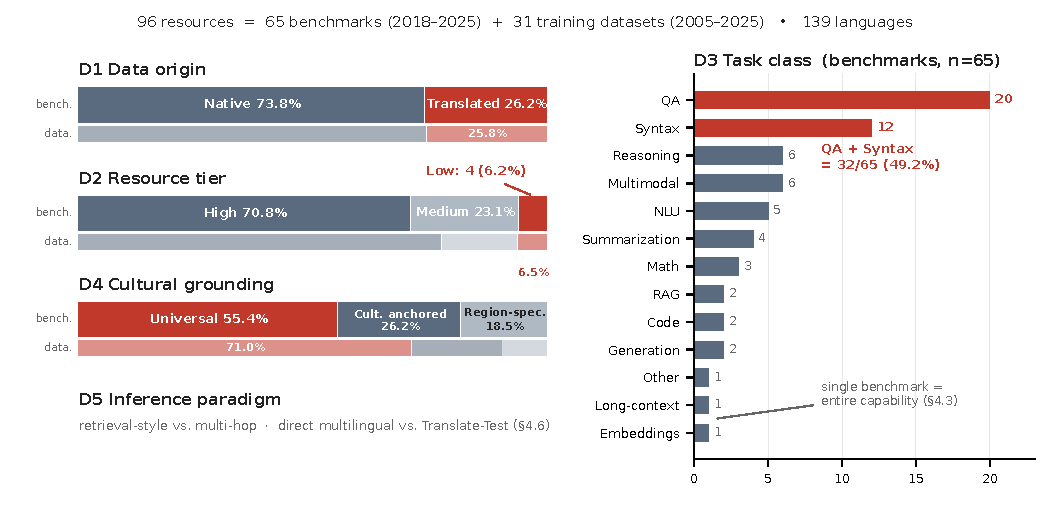
\includegraphics[width=\textwidth]{fig1_landscape.pdf}
\caption{Distribution of the 65 multilingual evaluation benchmarks across four taxonomy dimensions. Hatched red bars mark the imbalance each panel documents: reliance on translated data (A), near-absence of low-resource evaluation (B), concentration of effort in QA and syntax (C), and the majority of benchmarks that are culturally non-specific (D).}
\label{fig:landscape}
\end{figure*}
 
\subsection{A Pervasive Skew Toward High-Resource Languages}
Only 4 of 65 benchmarks (6.2\%)---and 2 of 31 datasets (6.5\%)---center low-resource languages, while 70.8\% of benchmarks and 77.4\% of datasets target predominantly high-resource ones (Table~\ref{tab:profile}). The language-level view is starker (Table~\ref{tab:languages}): English appears in 37 of 65 benchmarks, and coverage collapses past a short head---every language outside the twenty most-covered appears in at most 13 benchmarks. Nominal breadth also flatters the field: multi-way parallel suites such as BELEBELE's 122 language variants \cite{bandarkar2023belebele} multiply coverage by translating a single task---breadth without native depth.
 
The corpus documents what this skew costs. Where benchmarks do reach beyond the head, measured capability drops sharply: MMLU-ProX reports declines of up to 24.3\% for low-resource languages across 36 evaluated LLMs \cite{xuan2025mmluprox}; specialized code models collapse on low-resource and non-Python settings in mHumanEval's 204-language extension \cite{raihan2025mhumaneval}; and in multilingual long-context evaluation, gaps \emph{widen} as context grows, with English ranking only sixth---behind Polish---at long contexts \cite{kim2025oneruler}. These failure modes are invisible to the 93.8\% of benchmarks that rarely test where failure concentrates.
 
\begin{table}[t]
\centering
\small
\begin{tabular}{@{}rlr@{\hspace{1.4em}}rlr@{}}
\toprule
\# & Language & $n$ & \# & Language & $n$ \\
\midrule
1 & English & 37 & 11 & Korean & 26 \\
2 & Chinese & 35 & 12 & Italian & 25 \\
3 & Spanish & 31 & 13 & Vietnamese & 24 \\
4 & German & 30 & 14 & Thai & 23 \\
5 & French & 30 & 15 & Indonesian & 23 \\
6 & Russian & 30 & 16 & Turkish & 18 \\
7 & Arabic & 28 & 17 & Dutch & 18 \\
8 & Japanese & 28 & 18 & Czech & 15 \\
9 & Hindi & 27 & 19 & Polish & 14 \\
10 & Portuguese & 27 & 20 & Greek & 13 \\
\bottomrule
\end{tabular}
\caption{Benchmark coverage of the twenty most-covered languages ($n$ = number of the 65 benchmarks including the language). Each of the remaining 119 covered languages appears in at most 13 benchmarks; roughly 6{,}900 living languages appear in none.}
\label{tab:languages}
\end{table}
 
\subsection{Translated Foundations Distort Measurement}
More than a quarter of benchmarks (26.2\%) and datasets (25.8\%) are built on translated data---including the canonical cross-lingual evaluation suite: XNLI, XQuAD, MLQA, and PAWS-X are all translation-constructed \cite{conneau2018xnli,artetxe2020xquad,lewis2019mlqa,yang2019pawsx}. Translation was a rational bootstrapping strategy, but the corpus now contains direct evidence that it distorts the measurement instrument. Global-MMLU finds that 28\% of MMLU questions require culturally sensitive knowledge and 84.9\% of its geographic questions concern North America or Europe; re-evaluating 14 models on culturally sensitive versus culturally agnostic subsets \emph{changes model rankings} \cite{singh2024globalmmlu}. Benchmarks built from native sources depress inflated scores: GPT-4 scores 72.5\% on natively sourced ArabicMMLU---below its score on translated Arabic MMLU \cite{koto2024arabicmmlu}---and 59.95\% on Korean-native KMMLU, far below the $\sim$80\% pass mark of the source exams \cite{son2024kmmlu}, with the same pattern in Chinese and Turkish native suites \cite{li2023cmmlu,yuksel2024turkishmmlu}. On MultiLoKo's locally sourced questions in 31 languages, the best of 11 evaluated LLMs averages 34.4\% \cite{hupkes2025multiloko}. Score-level evidence converges: localized benchmarks correlate with human judgments at 0.68 versus 0.47--0.49 for translated ones \cite{wu2025bitter}. Where translation is unavoidable, rigorous pipelines with expert post-editing (e.g., IndicMMLU-Pro's back-translation and 13-reviewer verification) are the defensible middle path \cite{sankalp2025indicmmlupro}---but they remain a proxy for, not a substitute for, native evaluation.
 
\subsection{A Task Monoculture}
Question answering (30.8\%) and syntactic evaluation (18.5\%) together absorb 49.2\% of all benchmarks (Figure~\ref{fig:landscape}C), and the syntax count is partly template replication---BLiMP-style minimal pairs re-instantiated per language, up to 101 languages at once \cite{warstadt2023blimp,jumelet2025multiblimp}. Meanwhile the capabilities on which deployed systems actually depend are nearly unmeasured outside English: retrieval-augmented generation, code generation, and open-ended generation account for 3.1\% each; long-context understanding and embeddings for 1.5\% each---in several cases a \emph{single} benchmark stands for an entire capability \cite{kim2025oneruler,enevoldsen2025mmteb,liu2025xrag}. The supply side mirrors the imbalance: 64.5\% of training datasets are general pre-training corpora \cite{penedo2024fineweb,nguyen2023culturax,kudugunta2023madlad,laurencon2023roots}, leaving task-targeted multilingual training data scarce. Operationally, the field has defined ``multilingual capability'' as answering questions and judging grammaticality; on that definition, models can score well while remaining untested on the tasks users will actually give them.
 
\subsection{Cultural Grounding Is the Neglected Dimension}
A majority of benchmarks (55.4\%) and 71.0\% of datasets are ``universal''---designed to be culture-neutral, which in practice usually means cultural context has been stripped or inherited from Anglophone sources. Only 26.2\% of benchmarks are culturally anchored and 18.5\% region-specific. Language, however, is a cultural construct, and culturally agnostic evaluation certifies models that fail in situ: on the culturally curated ALM-bench, GPT-4o falls from 78.8\% overall to 50\% on Amharic \cite{vayani2025almbench}; the best model on ECLEKTIC achieves 41.6\% cross-lingual knowledge transfer \cite{goldman2025eclektic}; and SeaEval documents inconsistent answers to semantically equivalent queries across languages \cite{wang2024seaeval}. The countermovement---native school and professional exams (ArabicMMLU, CMMLU, KMMLU, TurkishMMLU), African-native IrokoBench \cite{adelani2024irokobench}, and participatory regional hubs such as SEACrowd \cite{lovenia2025seacrowd}---consistently reveals gaps that translated suites cannot, which is precisely the argument for funding more of it.
 
\subsection{The Supply Side Feeds the Same Gaps}
Auditing training datasets alongside benchmarks---which prior benchmark analyses do not---shows the two sides of the ecosystem reinforcing each other. Pre-training corpora dominate the supply (64.5\% of the 31 datasets), and the largest of them inherit the web's language distribution even at trillion-token scale \cite{penedo2024fineweb,nguyen2023culturax,kudugunta2023madlad,laurencon2023roots}. Translation and alignment corpora account for another 25.8\%. Multilingual \emph{instruction} data---the ingredient that turns a pre-trained model into a usable assistant---amounts to three datasets (9.7\%), of which only the participatory, human-curated Aya collection provides natively authored instructions at scale \cite{singh2024aya}. The pattern parallels the benchmark side: 74.2\% native, 77.4\% high-resource, 71.0\% culturally universal (Table~\ref{tab:profile}). Evaluation gaps and data gaps are the same gap seen from two directions, and closing one without the other leaves models that either cannot learn a capability or cannot prove they have it.
 
\subsection{Cross-Dimensional Dynamics}
Cross-referencing axes exposes three dynamics with direct practical consequences.
 
\textbf{The Translate-Test paradox.} Across independent low-resource evaluations, routing inputs through English outperforms direct multilingual inference: Indic-QA finds Translate-Test significantly better than direct inference, especially for low-resource Indic languages \cite{singh2024indicqa}; XNLI's translation-based baselines remain the strongest \cite{conneau2018xnli}; and on AmericasNLI's ten Indigenous languages, zero-shot cross-lingual transfer collapses to 30--50\% accuracy while translation-based approaches lead \cite{kann2022americasnli}. The seemingly inefficient pipeline winning is an indictment: native multilingual competence lags what aggregate leaderboards imply, and single-paradigm reporting hides the gap.
 
\textbf{Complexity is where multilinguality breaks.} The inference-paradigm axis shows measured competence degrading as tasks move from retrieval toward composition. Frontier models reach 55--62\% on cross-lingual RAG with monolingual retrieval but at most 58\% in genuinely multilingual retrieval, against human upper bounds of 85--92\%, frequently answering in the wrong language outright \cite{liu2025xrag}; cross-lingual knowledge transfer tops out at 41.6\% \cite{goldman2025eclektic}; and multilingual long-context aggregation tasks remain essentially unsolved, with under 1\% accuracy on the hardest variant \cite{kim2025oneruler}. Benchmarks confined to retrieval-style QA---the plurality of the corpus---systematically overstate how robust ``multilingual'' capability is.
 
\textbf{Scale is not a language policy.} Larger models lift averages without closing gaps: BenchMAX finds English--non-English gaps persist across model sizes \cite{huang2025benchmax}; P-MMEval shows measured transfer depends on the benchmark's language of origin \cite{zhang2025pmmeval}; test-time scaling gains are English-centric (+20 points on AIME vs.\ +1.9 averaged elsewhere) \cite{son2025mclm}; and multilingual chain-of-thought emerges only at extreme scale \cite{shi2022mgsm}. Waiting for scale to deliver equity is not a strategy.
 
\textbf{The surge is steerable.} Benchmark creation accelerated sharply in 2024--2025, and the fastest-growing thread is exactly the corrective one: natively sourced, culturally grounded, often community-built resources \cite{singh2024aya,lovenia2025seacrowd,adelani2024irokobench,enevoldsen2025mmteb}. The imbalances we quantify are not destiny; they are a snapshot of momentum that the community can redirect while the paradigm is still forming.
 
\section{From Diagnosis to Action}
The taxonomy is built to be used, not admired. We identify its users and translate each finding into a recommendation.
 
\textbf{Benchmark builders} can treat the five axes as a coverage card at design time and target empty cells directly: low-resource $\times$ reasoning, low-resource $\times$ long-context, region-specific $\times$ anything beyond QA. \textbf{Funders and program officers} gain quantified evidence for allocating scarce annotation budgets toward native data creation rather than further translation of saturated high-resource suites. \textbf{Model developers and auditors} can require evaluation-provenance disclosure---the native/translated share, cultural-specificity mix, and inference paradigm behind a claimed ``multilingual'' score---before accepting deployment claims for a region. \textbf{Language communities and regional consortia} can use the corpus to locate what exists for their languages and the taxonomy to name what is missing, converting absence into a fundable agenda---following the participatory models of Aya, SEACrowd, and IrokoBench \cite{singh2024aya,lovenia2025seacrowd,adelani2024irokobench}.
 
The stakes are practical, not academic. Multilingual models are already procured for education, public-health information, and government services in regions whose languages the certifying evaluations never natively tested; a system that scores well on translated, culture-stripped suites can still misinform a farmer in Amharic or a patient in Quechua while its leaderboard entry says otherwise (\S4.4--\S4.6). As governments and institutions write language requirements into AI procurement and national AI strategies, \emph{evaluation provenance}---what a ``multilingual'' claim was actually measured on---belongs in those requirements. The taxonomy supplies the vocabulary and the released annotations supply the evidence base for writing them.
 
The findings support five recommendations. \textbf{R1:} Prioritize natively sourced, culturally grounded benchmark creation in low-resource tiers, where 6.2\% coverage meets the largest measured performance drops (\S4.1, \S4.4). \textbf{R2:} Treat translated benchmarks as transitional scaffolding: label data origin explicitly, and report native-source results wherever both exist (\S4.2). \textbf{R3:} Diversify the task portfolio beyond QA and syntax toward reasoning, generation, retrieval, and long-context capabilities that deployment depends on (\S4.3). \textbf{R4:} Report both direct multilingual and Translate-Test performance; the gap between them is itself a diagnostic of native competence (\S4.5). \textbf{R5:} Adopt the five axes as a reporting standard for new evaluation resources---a datasheet for benchmarks---so the next generation of resources is born documented (\S3).
 
Our annotations are released in machine-readable form to support integration with dataset hubs and leaderboard metadata, and we commit to maintaining the corpus as a living resource with community refinement. \authnote{adjust this sentence to match what you will actually release/maintain.}
 
\section{Limitations}
Our corpus is a curated snapshot of a fast-moving field, not an exhaustive census; the five-axis annotation involves judgment, which we mitigate with public classification criteria and released annotations open to community correction \authnote{+ IAA statistic if available}. The taxonomy records the \emph{existence} and structure of resources, not their adoption or item-level quality. Finally, the performance dynamics in \S4 synthesize results reported by the primary studies under heterogeneous protocols; they are observational evidence, not controlled re-evaluations.
 
\section{Conclusion}
We introduced a five-dimensional taxonomy of multilingual AI evaluation, applied it to 96 resources, and quantified the field's structural imbalances: a 6.2\% share for low-resource languages, a quarter of benchmarks built on translation, half of all effort spent on two task families, and a majority of resources stripped of cultural grounding. These are measurements of an infrastructure that currently certifies ``multilingual'' AI for a world it does not represent. By reframing evaluation as foundational infrastructure---mapped, documented, and steerable---this work provides the evidence base for building AI that is not just multilingual in theory but globally reliable and culturally inclusive in practice.



\bibliography{aaai2027}

% Check whether the conference requires a reproducibility checklist to be included in the paper.
% If so, you can uncomment the following line and ajust the path to include it.
% \input{ReproducibilityChecklist.tex}

\end{document}
